\documentclass[11pt,a4paper,twocolumn,landscape]{article}
\synctex=1
\usepackage[utf8]{inputenc}
\usepackage[margin=1cm,left=0.5cm]{geometry}
\usepackage{graphicx}
%\usepackage{verbatim}
\usepackage{listings}
\usepackage{multicol}
\usepackage{textcomp}
\usepackage{courier}
\usepackage[hangul]{kotex}
\linespread{1}

\begin{document}
\pagenumbering{gobble}

\begin{center}
	\vspace*{2cm}
	{\Huge 시스템 소프트웨어
		\vspace{1cm}
		
실습 과제\\}
	\vspace{3cm}	
	
	\LARGE
	\begin{tabular}{rl}
		학번 : & 2016110056\\ 
		학과 : & 불교학부 \\
		이름 : & 박승원\\
		날짜 : & \today
	\end{tabular}
	\vspace{1cm}
	
	\includegraphics[width=0.1\textwidth]{logo.jpg}
	
\end{center}
\newpage
\noindent
\lstset{columns=flexible, tabsize=4, frame=single, showstringspaces=false, breaklines=true, upquote=true, basicstyle=\ttfamily\scriptsize}
\begin{enumerate}


\lstset{language=[x86masm]Assembler}
%\begin{multicols}{2}
\item 다음에 주어진 SIC/XE 프로그램을 입력하고, 실습하시오.(LISTFILE의 내용을 참고해서 각 label의 주소를 파악하고, 실행하면서 메모리와 register 들의 값의 변화를 관찰한다.)


\lstinputlisting{4.s}
1번 문제의 생성된 목적코드
\lstinputlisting{4.o}
각 실행 라인에서의 레지스터와 데이터의 값.
\lstinputlisting{1.txt}
레지스터를 보면 PC가 순환하는 것과 데이터의 값이 누적되는 것을 확인할 수 있다.\\
$4\rightarrow 7\rightarrow 9\rightarrow a$
\\
\item newd의 위치에서부터 차례대로 저장되어 있는 5개의 데이터 \{2,2,2,2,2\}을 모두 합하여 sum2에 저장하는 프로그램을 작성하고, 실습하시오.(위 프로그램을 수정한다.)
프로그램의 작성 예..

\lstinputlisting{5.s}
2번 문제의 생성된 목적코드 
\lstinputlisting{5.o}
각 실행 라인에서의 레지스터와 데이터의 값.
\lstinputlisting{2.txt}
마찬가지로 PC가 순환하는 것과 값이 누적되는 것을 확인할 수 있다. 그리고, 마지막에는 a, 십진수로 10이 결과로 나오는 것을 확인할 수 있다.
%\end{multicols}
\newpage
컴파일 후의 심볼테이블(푸른 테두리)과 실행 전후의 데이터 영역(붉은 색이 구하고자 하는 값).\\
\vspace{1cm}
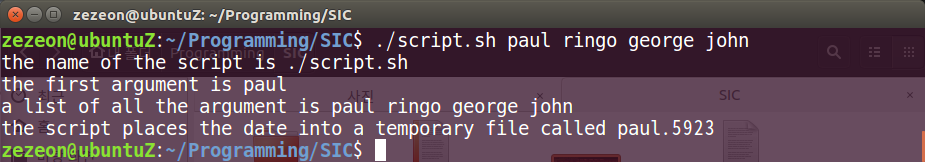
\includegraphics[width=0.5\textwidth]{2.png}
		\lstset{language=C}
\newpage
지난 시간에 만든 것에 X레지스터의 값을 더하여 메모리를 액세스하는 부분과 COMP, JLT를 더하였다.
약간의 수정을 가하여, 에뮬레이터를 조금 변경하였다.

\begin{lstlisting}[language=C++]
void SIC::COMP(short addr) 
{
	int n = fetch(addr);
	int a = A;
	if(a < n) SW.opcode = 1;
	else SW.opcode = 0;
}

void SIC::JLT(short addr) 
{
	if(SW.opcode == 1) PC.address = addr-3;
}

void SIC::ADDX(short addr)
{
	int a = A;
	int x = X;
	int k = fetch(addr + x);
	A = a + k;
}

\end{lstlisting}


\end{enumerate}

{\Huge소감}
\indent
수업시간에 배우지 않은 부분인 조건분기와 X레지스터의 값을 참조하여 더하는 명령어가 나와 애를 먹었다.
조건문은 잠정적으로 SW레지스터의 opcode를 1로 셋팅하는 것으로 설정하고, addx라는 opcode를 추가하여 프로그램을 만들어 보았다. 
소오스가 끝에 trailing하는 스페이스가 있을 경우 제대로 작동하지 않는 점도 발견하였다. 
\end{document}
